% !TeX spellcheck = en_US
%
%
% v 2.3  Feb 2019   Volker RW Schaa
%		# changes in the collaboration therefore updated file "jacow-collaboration.tex"
%		# all References with DOIs have their period/full stop before the DOI (after pp. or year)
%		# in the author/affiliation block all ZIP codes in square brackets removed as it was not 
%         understood as optional parameter and ZIP codes had bin put in brackets
%       # References to the current IPAC are changed to "IPAC'19, Melbourne, Australia"
%       # font for "url" style changed to "newtxtt" as it is easier to distinguish "O" and "0"
%
\documentclass[letter,
               %boxit,        % check whether paper is inside correct margins
               %titlepage,    % separate title page
               %refpage       % separate references
               %biblatex,     % biblatex is used
               keeplastbox,   % flushend option: not to un-indent last line in References
               %nospread,     % flushend option: do not fill with whitespace to balance columns
               %hyphens,      % allow \url to hyphenate at "-" (hyphens)
               %xetex,        % use XeLaTeX to process the file
               %luatex,       % use LuaLaTeX to process the file
               ]{jacow}
%
% ONLY FOR \footnote in table/tabular
%
\usepackage{pdfpages,multirow,ragged2e} %
%
% CHANGE SEQUENCE OF GRAPHICS EXTENSION TO BE EMBEDDED
% ----------------------------------------------------
% test for XeTeX where the sequence is by default eps-> pdf, jpg, png, pdf, ...
%    and the JACoW template provides JACpic2v3.eps and JACpic2v3.jpg which
%    might generates errors, therefore PNG and JPG first
%
\makeatletter%
	\ifboolexpr{bool{xetex}}
	 {\renewcommand{\Gin@extensions}{.pdf,%
	                    .png,.jpg,.bmp,.pict,.tif,.psd,.mac,.sga,.tga,.gif,%
	                    .eps,.ps,%
	                    }}{}
\makeatother

% CHECK FOR XeTeX/LuaTeX BEFORE DEFINING AN INPUT ENCODING
% --------------------------------------------------------
%   utf8  is default for XeTeX/LuaTeX
%   utf8  in LaTeX only realises a small portion of codes
%
\ifboolexpr{bool{xetex} or bool{luatex}} % test for XeTeX/LuaTeX
 {}                                      % input encoding is utf8 by default
 {\usepackage[utf8]{inputenc}}           % switch to utf8

\usepackage[USenglish]{babel}


%
% if BibLaTeX is used
%
\ifboolexpr{bool{jacowbiblatex}}%
 {%
  \addbibresource{jacow-test.bib}
  \addbibresource{biblatex-examples.bib}
 }{}
\listfiles

%%
%%   Lengths for the spaces in the title
%%   \setlength\titleblockstartskip{..}  %before title, default 3pt
%%   \setlength\titleblockmiddleskip{..} %between title + author, default 1em
%%   \setlength\titleblockendskip{..}    %afterauthor, default 1em

\begin{document}

\title{preparation OF papers for \NoCaseChange{JACoW} conferences\thanks{Work supported by ...}}

\author{A. N. Author\thanks{email address}, H. Coauthor, Name of Institute or Affiliation, City, Country \\
		P. Contributor\textsuperscript{1}, Name of Institute or Affiliation, City, Country \\
		\textsuperscript{1}also at Name of Secondary Institute or Affiliation, City, Country}
	
\maketitle

%
\begin{abstract}
   Many conference series have adopted the same standards
   for electronic publication and have joined the Joint
   Accelerator Conferences Website (JACoW) collaboration
   for the publication of their proceedings. This document
   describes the common requirements for the submission of
   papers to these conferences. Please consult individual
   conference information for page limits, method of electronic
   submission, etc. It is not intended that this should
   be a tutorial in word processing; the aim is to explain the
   particular requirements for electronic publication at
   www.JACoW.org. The abstract itself is to act as a stand-alone
   entity and, as such, should not include citations. Any acronyms 
   should be expanded on their first occurrence, both in the 
   abstract and in the rest of the paper. 
   The abstract itself is to act as a stand-alone entity and, 
   as such, should not include citations. Any acronyms should 
   be expanded on their first occurrence, both in the abstract 
   and in the rest of the paper.
\end{abstract}


\section{SUBMISSION OF PAPERS}
Each author should submit the PDF file and all source
files (text and figures) to enable the paper to be
reconstructed if there are processing difficulties.

\section{MANUSCRIPTS}
Templates are provided for recommended software and
authors are advised to use them. Please consult the
individual conference help pages if questions arise.

\subsection{General Layout}

These instructions are a typical implementation of the
requirements. Manuscripts should have:
\begin{Itemize}
    \item  Either A4 (\SI{21.0}{cm}~$\times$~\SI{29.7}{cm}; \SI{8.27}{in}~$\times$~\SI{11.69}{in}) or US
           letter size (\SI{21.6}{cm}~$\times$~\SI{27.9}{cm}; \SI{8.5}{in}~$\times$~\SI{11.0}{in}) paper.
    \item  Single-spaced text in two columns of \SI{82.5}{mm} (\SI{3.25}{in}) with \SI{5.3}{mm}
           (\SI{0.2}{in}) separation. More recent versions of Microsoft Word have a default spacing of 1.5 lines;
           authors must change this to 1 line.
    \item  The text located within the margins specified in Table~\ref{tab:margins}.
\end{Itemize}
\begin{table}[!hbt]
   \centering
   \caption{Margin Specifications}
   \begin{tabular}{lcc}
       \toprule
       \textbf{Margin} & \textbf{A4 Paper}                      & \textbf{US Letter Paper} \\
       \midrule
           Top         & \SI{37}{mm} (\SI{1.46}{in})            & \SI{0.75}{in} (\SI{19}{mm})        \\ %[3pt]
          Bottom       & \SI{19}{mm} (\SI{0.75}{in})            & \SI{0.75}{in} (\SI{19}{mm})        \\ %[3pt]
           Left        & \SI{20}{mm} (\SI{0.79}{in})            & \SI{0.79}{in} (\SI{20}{mm})        \\ %[3pt]
           Right       & \SI{20}{mm} (\SI{0.79}{in})            & \SI{1.02}{in} (\SI{26}{mm})        \\
       \bottomrule
   \end{tabular}
   \label{tab:margins}
\end{table}

\subsection{Fonts}

In order to produce good Adobe Acrobat PDF files, authors
using the `jacow' \LaTeX{} template are asked to use only the fonts
defined in the `jacow' class file (v2.3 of 2019/01/15) in standard, 
bold (i.\,e., \verb|\textbf|) or italic (i.\,e., \verb|\textit|) form and
symbols from the standard set of fonts. In Word use only
Symbol and, depending on your platform, Times or Times New Roman
fonts in standard, bold or italic form.

The layout of the text on the page is illustrated in
Fig.~\ref{fig:paper_layout}. Note that the paper's title and the author list should
be the width of the full page. Tables and figures may span
the whole \SI{170}{mm} page width, if desired (see Fig.~\ref{fig:jacow_team}), but
if they span both columns, they should be placed at either
the top or bottom of a page to ensure proper flow of the
text (which should flow from top to bottom in each column).

\begin{figure}[!htb]
   \centering
   \includegraphics*[width=.7\columnwidth]{JACpic_mc}
   \caption{Layout of papers.}
   \label{fig:paper_layout}
\end{figure}

\begin{figure*}[!tbh]
    \centering
    \includegraphics*[width=\textwidth]{JACpic2}

    \caption{Example of a full-width figure showing the JACoW Team at their annual
    	     meeting in December 2018. This figure has a multi-line caption that has to be
    	     justified rather than centred.} %US
    \label{fig:jacow_team}
\end{figure*}

\subsection{Title and Author List}

The title should use \SI{14}{pt} bold uppercase letters and be centred on the page.
Individual letters may be lowercased to avoid misinterpretation (e.\,g., mW, GeV, 
SPring-8, SwissFEL).
To include a funding support statement, put an asterisk after the title and
the support text at the bottom of the first column on page~1---in Word,
use a text box; in \LaTeX, use $\backslash$\texttt{thanks}. See also the
subsection on footnotes.

The names of authors, their organizations/affiliations and
postal addresses should be grouped by affiliation and
listed in \SI{12}{pt} upper- and lowercase letters. The name of
the submitting or primary author should be first, followed
by the coauthors, alphabetically by affiliation. Where
authors have multiple affiliations, the secondary affiliation
may be indicated with a superscript, as shown in the
author listing of this paper. See \textbf{ANNEX~A} for further examples.

\subsection{Section Headings}

Section headings should not be numbered. They should
use  \SI{12}{pt}  bold  uppercase  letters  and  be  centered  in  the
column. All section headings should appear directly above
the text---there should never be a column break between a heading and the
following paragraph.

\subsection{Subsection Headings}

Subsection  headings  should  not  be  numbered.
They should use \SI{12}{pt} italic letters and be left aligned in the column.
Subsection headings use Title Case (or Initial Caps)
and should appear directly above the text---there should never be a column break
between a subheading and the following paragraph.

\subsubsection{Third-level Headings} These should use \SI{10}{pt} bold
letters and be run into the paragraph text. In \LaTeX{} these headings are
created with \LaTeX's \verb|\subsubsection| command.
In the Word templates authors must bold the heading text themselves.
This heading should be used sparingly. See Table~\ref{tab:styles}
for its style details.

\subsection{Paragraph Text}

Paragraphs should use \SI{10}{pt} font and be justified (touch each side) in
the column. The beginning of each paragraph should be indented
approximately \SI{0.33}{cm} (\SI{0.13}{in}). The last line of a paragraph should not be
printed by itself at the beginning of a column nor should the first line of
a paragraph be printed by itself at the end of a column.

\subsection{Figures, Tables, and Equations}

Place figures and tables as close to their place of mention as
possible. Lettering in figures and tables should be large enough to
reproduce clearly. Use of non-approved fonts in figures can lead to
problems when the files are processed. \LaTeX{} users should be sure to use
non-bitmapped versions of Computer Modern fonts in equations (Type\,1 PostScript
or OpenType fonts are required. Their use is described in the help 
pages of the JACoW website\cite{jacow-help}).

Each figure and table must be numbered in ascending
order (1, 2, 3, etc.) throughout the paper. 
Figure captions are placed below figures, and table
captions are placed above tables.

Figure captions are formatted as shown in Figs.~\ref{fig:paper_layout} and \ref{fig:jacow_team},
while table captions take the form of a heading,
with initial letters of principle words, capitalized, and
without a period at the end (see Tables~\ref{tab:margins} and~\ref{tab:styles}).
Any reference to the contents of the table should be made from
the body of the paper rather than from within the table
caption itself.

Single-line captions are centered in the column, while captions
that span more than one line should be justified.
The \LaTeX{} template uses the “booktabs” package to
format tables.

When referring to a figure from within the text, the
convention is to use the abbreviated form [e.\,g., Fig.~1]
\emph{unless} the reference is at the start of the sentence, in
which case “Figure” is written in full. Reference to a
table, however, is never abbreviated [e.\,g., Table~1].


If a displayed equation needs a number (i.\,e., it will be
referenced), place it in parentheses, and flush with the
right margin of the column. The equation itself should be
indented and centered, as far as is possible:
\begin{equation}\label{eq:label}
    C_B=\frac{q^3}{3\epsilon_{0} mc}=\SI{3.54}{\micro eV/T}
\end{equation}

When referencing a numbered equation, use the word
“Equation” at the start of a sentence, and the abbreviated
form, “Eq.”, if in the text. The equation number is placed
in parentheses [e.\,g., Eq.~\eqref{eq:label}], which can be 
achieved in \LaTeX{} using \verb|\eqref{eq:label}|.

\subsection{Units}
	
Units should be written using the standard, roman font,
not the italic font, as shown in Eq.~\eqref{eq:label}.
An unbreakable space should precede a unit (in \LaTeX{} use a “\verb|\,|”,
the template uses the “siunitx” package to format units).
Some examples are: \SI{3}{keV},
\SI{100}{kW}, \SI{7}{µm}. When a unit appears in a hyphenated,
compound adjective that precedes a noun, it takes on the
singular form, e.\,g., the 3.8-meter long undulator.

\subsection{References}
%
% References examples given here are not formatted using \cite as there
%			 are only reference numbers [1] and [2] in the template
%
All bibliographical and web references should be numbered and listed at the
end of the paper in a section called \textbf{REFERENCES}. When citing a
reference in the text, place the corresponding reference number in square
brackets~[1]. The reference citations in the text should be numbered
in ascending order. Multiple citations should appear in
the same bracket~[3, 4] and
with ranges where appropriate~[1--4, 10].

A URL or DOI may be included as part of a reference, but its
hyperlink should NOT be added. The usual practice is to
use a monospaced font for the URL so as to help distinguish
it from normal text. In \LaTeX{} the “url” package is used with its 
default font now being switched to ``newtxtt'' which offers
a better distinction between ``\texttt{O}'' and ``\texttt{0}''.

For authors to properly cite the resources used when researching
their papers is an obligation. In the interest of
promoting uniformity and complete citations, the IEEE
Editorial Style for Transactions and Journals, which itself 
adheres to the Chicago Manual of Style, has been adopted~\cite{IEEE}. 
When citing a periodical, the official abbreviation of the journal 
should be used\cite{journal-abbreviations}.
Please consult the appended material, \textbf{ANNEX~B},
for details. The onus is on authors to pay attention to
the details of the said style to ensure complete, accurate
and properly formatted references.

  \begin{table}[h!b]
	\setlength\tabcolsep{3.5pt}
	\centering
	\caption{Summary of Styles}
	\label{tab:styles}
	\begin{tabular}{llcc}
		\toprule
		\textbf{Style} & \textbf{Font}               & \textbf{Space}  & \textbf{Space} \\
		&                             & \textbf{Before} & \textbf{After} \\
		\midrule
		\textbf{PAPER}  & \SI{14}{pt}                 & \SI{0}{pt}      & \SI{3}{pt}  \\
		\textbf{TITLE}  & \textbf{UPPERCASE}          &                 &      \\
		& \textbf{EXCEPT FOR}         &                 &      \\
		& \textbf{REQUIRED lowercase} &                 &      \\
		& \textbf{letters}            &                 &      \\
		& \textbf{Bold}               &                 &      \\[5pt]
		%\midrule
		Author list  & \SI{12}{pt}                 & \SI{9}{pt}      & \SI{12}{pt} \\
		& UPPER- and lowercase        &                 &      \\[5pt]
		%\midrule
		\textit{Abstract} & \SI{12}{pt}                 & \SI{0}{pt}      & \SI{3}{pt} \\
		\textit{Title}  & \textit{Initial Caps}       &                 &      \\
		& \textit{Italic}             &                 &      \\[5pt]
		%\midrule
		\textbf{Section}  & \SI{12}{pt}                 & \SI{9}{pt}      & \SI{3}{pt}  \\
		\textbf{Heading}  & \textbf{UPPERCASE}          &                 &      \\
		& \textbf{bold}               &                 &      \\[5pt]
		%\midrule
		\textit{Subsection} & \SI{12}{pt}                 & \SI{6}{pt}      & \SI{3}{pt}  \\
		\textit{Heading}
                             & \textit{Initial Caps}       &                 &      \\
		& \textit{Italic}             &                 &      \\[5pt]
		%\midrule
		\textbf{Third-level} & \SI{10}{pt}                 & \SI{6}{pt}      & \SI{0}{pt}  \\
		\textbf{Heading}     
                            & \textbf{Initial Caps}       &                 &      \\
		& \textbf{Bold}               &                 &      \\[5pt]
		%\midrule
		Figure        & \SI{10}{pt}                 & \SI{3}{pt}      & $\ge$\SI{3}{pt}  \\
		Captions      &                             &                 &      \\[5pt]
		%\midrule
		Table         & \SI{10}{pt}                 & $\ge$\SI{3}{pt} & \SI{3}{pt}  \\
		Captions	  &                             &                 &      \\[5pt]
		%\midrule
		Equations     & \SI{10}{pt} base font       & $\ge$\SI{6}{pt}     & $\ge$\SI{6}{pt} \\[5pt]
		%\midrule
		References      & \SI{9}{pt}				& \SI{0}{pt}      & \SI{3}{pt} \\
        when $\le9$ 	& \verb|\bibliography{9}|	&                 &  \\[5pt]
        Refs. $\ge10$ 	& \SI{9}{pt}				& \SI{0}{pt}      & \SI{3}{pt}  \\
                		& \verb|\bibliography{99}|	&    &    \\
		\bottomrule   %\SI{0.25}{in}
	\end{tabular}
\end{table}

\subsection{Footnotes}

Footnotes on the title and author lines may be used for acknowledgments
and e-mail addresses. A non-numeric sequence of characters (*, \#,
\dag, \ddag, \P) should be used to indicate the footnote.
These “pseudo footnotes” should only
appear at the bottom of the first column on the first page.

Any other footnote in the body of the paper should
use the normal numeric sequencing (i.\,e., 1, 2, 3)
and appear at the bottom of the same column in which
it is used.  All footnotes are of 8pt font size.

\subsection{Acronyms}

Acronyms should be defined the first time they appear, 
both in the abstract and in the rest of the paper. 

\section{STYLES}

Table~\ref{tab:styles} summarizes the fonts and spacing used in the styles of
a JACoW template. In \LaTeX, these 
are implemented in the “jacow” class file.

\section{PAGE NUMBERS}

\textbf{DO NOT include any page numbers}. They will be added
when the final proceedings are produced.

\section{TEMPLATES}

Template documents for the recommended word processing
software are available from the JACoW website~\cite{jacow-help}
and exist for \LaTeX, Microsoft Word (Mac and PC)
and LibreOffice/Apache OpenOffice for US letter and A4
paper sizes. Use the correct template for your paper size and
platform.

Fonts are embedded by default with pdf\LaTeX. Using \LaTeX{} with `dvips', 
make sure that `ps2pdf' has the option \texttt{-dEmbedAllFonts=true}'.
Fonts of included figure graphics in PDF or EPS are often not embedded. 
So make sure that this done when generating them or reprocess them 
in `Ghostscript' with the switch \texttt{-dEmbedAllFonts=true}' set.

\flushcolsend

\section{CHECKLIST FOR ELECTRONIC PUBLICATION}
Authors are requested to go over the following checklist for electronic publication:
\begin{Itemize}
	\item  Use only Times or Times New Roman (standard, bold or italic) and Symbol
	fonts for text, \SI{10}{pt} except references, which should be \SI{9}{pt}.
	
	\item  Figures should use Times or Times New Roman (standard, bold or italic) and
	Symbol fonts when possible---\SI{6}{pt} minimum, with fonts embedded.
	\item  Check that citations to references appear in sequential order and
	that all references are cited.
	\item  Check that the PDF file prints correctly.
	\item  Check that there are no page numbers.
	\item  Check that the margins on the printed version are within \SI{\pm1}{mm}
	of the specifications.
	\item  \LaTeX{} users can check their margins by invoking the
	\texttt{boxit} option.
\end{Itemize}

Please also check the list of common oversights which can be found in \textbf{ANNEX C}.

\section{CONCLUSION}

Any conclusions should be in a separate section directly preceding
the \textbf{ACKNOWLEDGMENTS}, \textbf{APPENDIX}, or \textbf{REFERENCES} sections, in that
order.

\section{ACKNOWLEDGMENTS}
Any acknowledgement should be in a separate section directly preceding
the \textbf{REFERENCES} or \textbf{APPENDIX} section.


\section{APPENDIX}
Any appendix should be in a separate section directly preceding
the \textbf{REFERENCES} section. If there is no \textbf{REFERENCES} section,
this should be the last section of the paper.

%
% only for "biblatex"
%
\ifboolexpr{bool{jacowbiblatex}}%
	{\printbibliography}%
	{%
	% "biblatex" is not used, go the "manual" way
	
	%\begin{thebibliography}{99}   % Use for  10-99  references
	\begin{thebibliography}{9} % Use for 1-9 references
	
	\bibitem{jacow-help}
		JACoW,
		\url{http://www.jacow.org}
	
	\bibitem{IEEE}
		\textit{IEEE Editorial Style Manual},
		IEEE Periodicals, Piscataway,
		NJ, USA, Oct. 2014, pp. 34--52.

	\bibitem{journal-abbreviations}
	\url{https://woodward.library.ubc.ca/researchhelp/journal-abbreviations/}

	\end{thebibliography}
} % end \ifboolexpr

%
% for use as JACoW template the inclusion of the ANNEX parts have been commented out
% to generate the complete documentation please remove the "%" of the next two commands
% 
%%%%\newpage

%%%%%
% !TeX spellcheck = en_US
%
\twocolumn[\vspace*{-1.8ex}\section{ANNEX A:\endgraf FORMATTING OF AUTHORS AND AFFILIATIONS}\vspace*{\baselineskip}]

\flushcolsend

The names of authors, their organizations/affiliations
and postal addresses should be grouped by affiliation and
listed in \SI{12}{pt} upper- and lowercase letters. The name of
the submitting or primary author should be first, followed
by the coauthors, alphabetically by affiliation. If the
author list for a given affiliation spans multiple lines,
please be sure to break the line in a manner that does not
split the author’s initials from the author’s last name. This
is easily done by placing unbreakable spaces between the
initials and last name. The affiliation name and address
are also best kept together on the same (but not necessarily
separate) line, wherever possible. (See, for example,
the entry for GSI in the following). In cases where authors
have multiple affiliations, the secondary affiliation is
inserted below the author/primary affiliation listing and is
indicated with a superscript, as shown in the following.


Footnotes on the title and author lines may be used for
acknowledgments and e-mail addresses, using a non-numeric
sequence of characters (\textsuperscript{*}, \textsuperscript{†},
\textsuperscript{‡}, \textsuperscript{§}, \textsuperscript{\P}
as generated by \LaTeX's \verb|\footnote| command).

For examples of the preferred formatting of authors and
affiliations, please consult the following list of JACoW
collaboration members.

For manuscripts submitted by large collaborations with
potentially many tens of authors and where, additionally,
there may be page number limitations, a format consisting
of the principle author’s name and institute, followed by
“on behalf of the \ldots\ collaboration”, is preferred.


\clearpage
%
% Include the title/author page of the JACoW Coolaboration
%
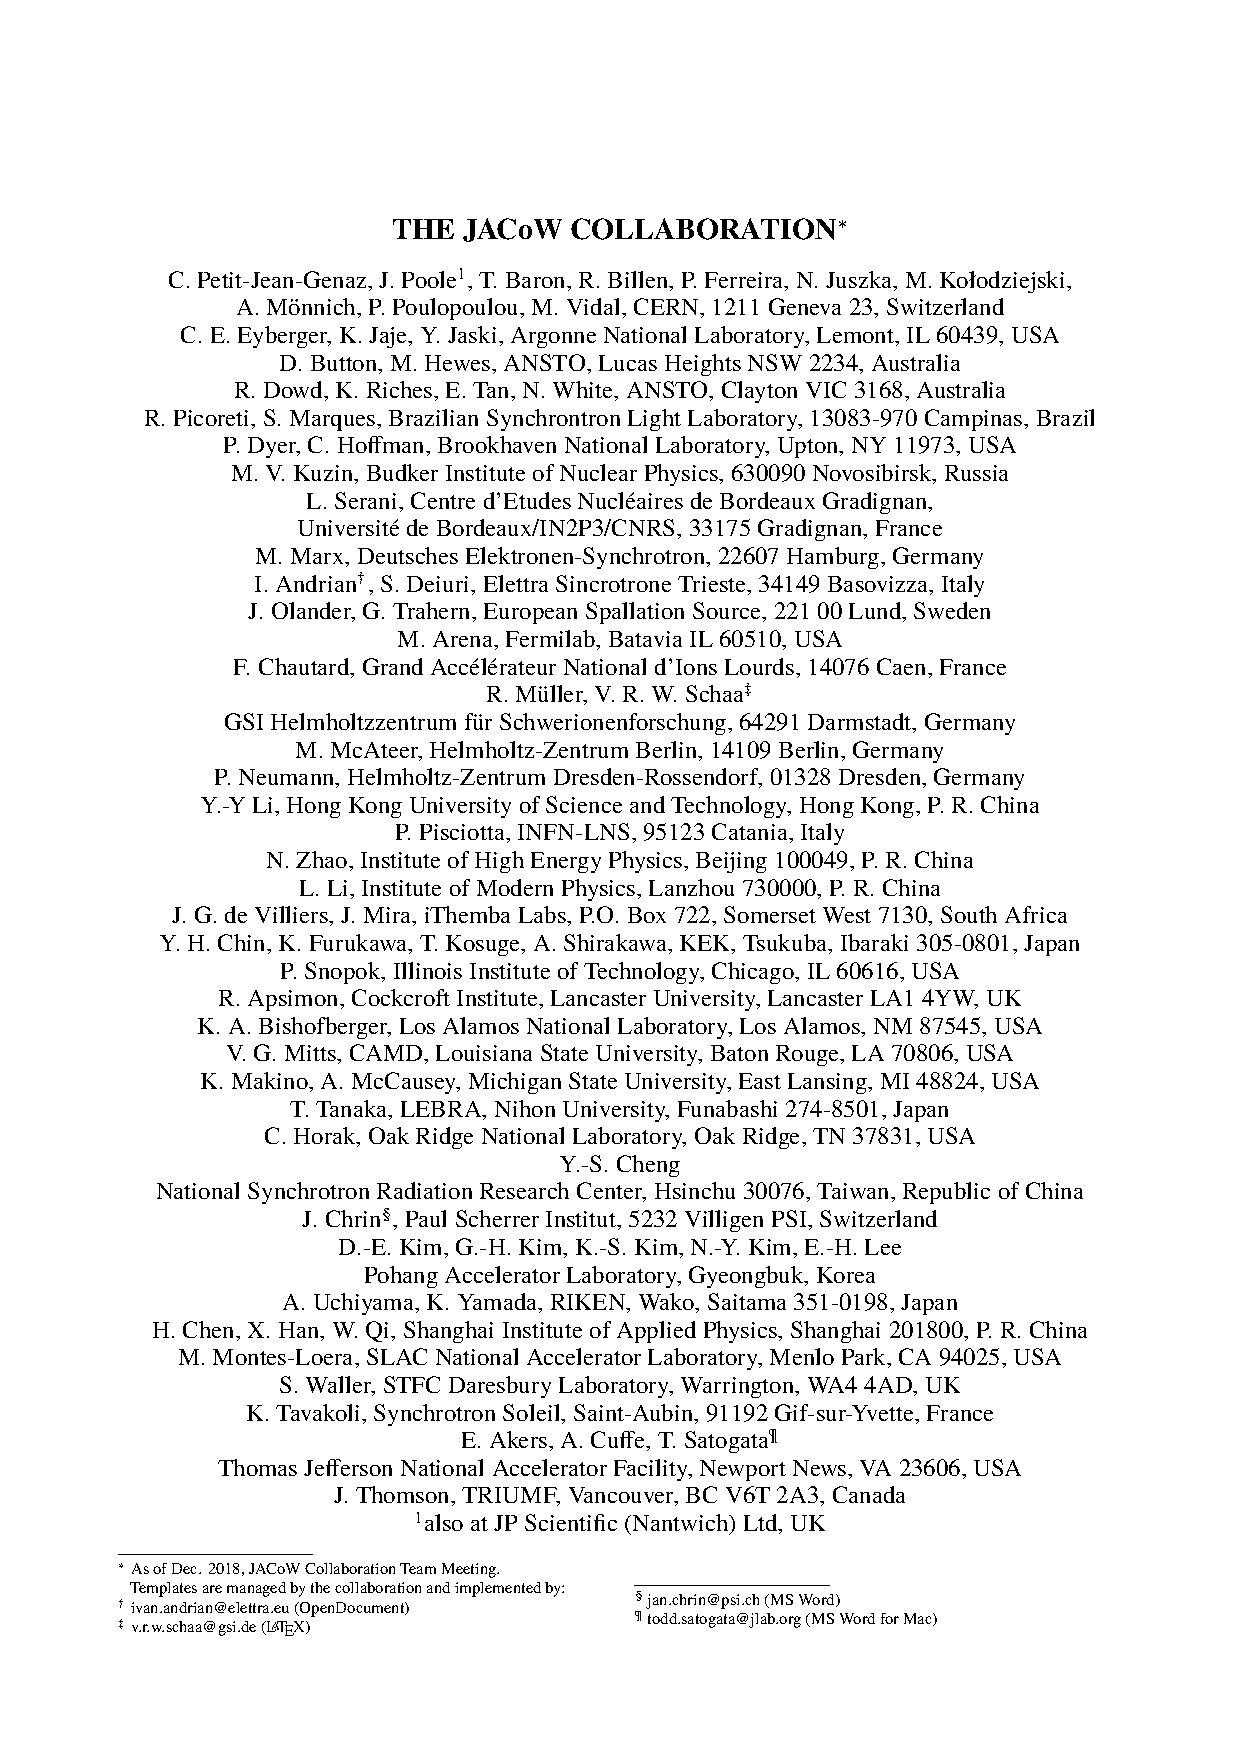
\includepdf[pages=-, noautoscale, pagecommand={}]{jacow-collaboration.pdf}{}

\clearpage

\twocolumn[\vspace*{-1.8ex}\section{ANNEX B:\endgraf IEEE REFERENCE STYLE GUIDE AS APPLIED TO \NoCaseChange{JACoW} PAPERS, \break PERIODICALS AND OTHER WORKS}\vspace*{\baselineskip}]

\subsection{Referencing JACoW Proceedings}

The format for published JACoW proceedings papers is detailed in the following 
and can also be readily deduced from Refs.~[1-3]. At the very minimum, sufficient 
information should be given to enable readers to clearly identify the paper and 
to facilitate its import into digital databases.
\vspace*{-.6\baselineskip}

\subsubsection{Author Listing} Careful attention should be given to the
placing of commas and the use of ‘and’ in the author list.
In particular, for the case of three or more authors
(as in [3]), a comma also follows the penultimate author.
The preference for ‘\emph{et al.}’\ takes precedence when the number
of authors becomes large (e.g., $>$6).
\vspace*{-.6\baselineskip}

\subsubsection{Paper Title} As is modern practice in references, the title
of the paper is written in sentence case, i.\,e., only the
initial letter of the first word in the title is capitalized.
Proper nouns, however, also have a capital. Capital letters
appearing in acronyms likewise remain unaltered
\vspace*{-.6\baselineskip}

\subsubsection{Conference Proceedings} The title of the proceedings is
written in title case in italics using standard abbreviations,
such as \emph{Int.} and \emph{Conf.} The preposition, ``in'', in normal
font, precedes the proceedings title. The location,
i.\,e., city, state (if USA), and country of the conference
venue, the month (three-letter abbreviation) and the year
the conference took place, is then listed. Finally, details
pertaining to the paper itself, such as the conference paper
ID, mandatory page numbers, and the digital object
identifier (DOI), if existing, are listed in the given order.
A monospaced font for the DOI is used so as to help
distinguish it from normal text. In \LaTeX{}
the ‘url’ package is used. The Word template uses the Liberation
Mono TrueType font (size 8 pt), or Lucida Sans Typewriter
font (size 7.5 pt) in earlier Word versions where the Liberation
Mono font may not be available. In LaTeX, the ‘url’
package is used with its default font now being switched to 
``newtxtt'' which offers a better distinction between 
``\texttt{O}'' and ``\texttt{0}''. The conference
paper ID is optional and may be included in the absence
of a DOI to facilitate a search through internet search
engines. DOIs have been assigned to all JACoW
publications appearing in recent proceedings and will
likewise be assigned to articles from conferences further
past, in due course. The use of DOIs is strongly
emphasized.

The complete or abbreviated form for citations, as
shown in the following section, is advocated. The former
is more informative to readers outside the immediate
conference sphere, and will further serve to avoid
potential ambiguities in cases where an acronym is not
unique. Both forms, however, when adhered to, ensure a
proper import into digital libraries and information
sources such as INSPIRE, Scopus, and Google Scholar.
Authors are also reminded to make a distinction between
papers published in JACoW proceedings (which have
page numbers and, in the case of recent publications,
DOIs) and those papers that may have been presented at
past JACoW conferences but were not published~[4].
References to contributions presented at the same
conference should be written as shown in [5]; the wording
“this conference” may be optionally appended.

\subsection{Referencing Periodicals and Other Sources}

The IEEE style is also shown for periodicals [6-11],
online sources [12], books [13, 14], internal reports [15],
theses [16], manuals or handbooks [17], patents [18] and
unpublished material [19, 20]. When citing a periodical,
only the official abbreviation of the journal should be used
[21]. Examples of correctly formatted references can also be 
found at the JACoW website, under ‘Formatting Citations’ which 
is reached through the ‘for Authors’ link.

\subsection{Alignment of References}

In the \LaTeX{} template, \verb|\bibliography{9}| is used for
when the total number of references is less than ten. This
should be changed to \verb|\bibliography{99}| if the number of
references is ten or more.

\patchcmd\thebibliography{\section*{REFERENCES\@mkboth {REFERENCES}{REFERENCES}}}{}{}{}
\section{PAPER PUBLISHED IN A CONFERENCE PROCEEDINGS}

\definecolor{jgreen}{cmyk}{0.81, 0.00, 0.97, 0.00}
\definecolor{jred}{cmyk}  {0.00, 0.99, 1.00, 0.00}
\definecolor{jgrepc}{cmyk}{0.74, 0.05, 1.00, 0.00}
\definecolor{jblue}{cmyk} {0.87, 0.54, 0.00, 0.00}
\definecolor{jvio}{cmyk}  {0.41, 0.82, 0.00, 0.00}
\definecolor{jbook}{cmyk} {0.28, 0.88, 0.79, 0.25}
\definecolor{jrept}{cmyk} {0.07, 0.70, 1.00, 0.00}
\definecolor{jmanu}{cmyk} {0.28, 0.77, 1.00, 0.23}
\definecolor{junpu}{cmyk} {0.00, 0.83, 0.65, 0.00}


\subsection{Complete Form}

\newcommand{\CCom}[2]{\newline\textcolor{#1}{[#2]}}
%\begin{thebibliography}{99}   % Use for  10-99  references
\begin{thebibliography}{9} % Use for 1-9 references
	
	\bibitem{item:1-1}
	A.~Alpha and B.~T.~Beta, “Novel techniques for future TeV electron accelerators,”
	in \textit{Proc.\ 9th Int.\ Particle Accelerator Conf.\ (IPAC’18)},
	Vancouver, BC, Canada, Apr.-May 2018.
	pp. 567-569. \url{doi:10.18429/JACoW-IPAC2017-PAPERID}
	\CCom{jgreen}{Conference Proceedings, two authors; DOI encouraged}

	\bibitem{item:1-2}
	A.~Alpha \emph{et al.},
	“A novel injector,” in \emph{Proc.\ 29th Linear Accelerator Conf.\ (LINAC’18)},
	Shanghai, China, Sep.\ 2018, pp.\ 27-31. %\newline
	\url{doi:10.18429/JACoW-LINAC2018-PAPERID}
	\CCom{jgreen}{Conference Proceedings, for six or more authors use \emph{et al.};	
		 DOI encouraged}
	
	\bibitem{item:1-3}	
	A.~Alpha, B.~T.~Beta, C.~Gamma, and D.~Delta,
	“An overview of control systems,”
	in \emph{Proc.\ 13th Int.\ Conf.\ on Accelerator and Large Experimental Physics Control Systems (ICALEPCS’11)}, Grenoble, France, Oct.\ 2011,
	paper TUP014, pp.\ 89--91.
	\CCom{jgreen}{Conference Proceedings, four authors; optional paper ID
	in the absence of a DOI}
\end{thebibliography}

\vspace*{-.5\baselineskip}
\subsection{Abbreviated Form}

\begin{thebibliography}{9} % Use for 1-9 references
	\bibitem{item:2-1}
	A.~Alpha and B.~T.~Beta, “Novel techniques for future TeV electron accelerators,”
	in \textit{Proc.\ IPAC’18}, Vancouver, BC, Canada, Apr.-May 2018,
	pp.\ 567-569. %\newline
	\url{doi:10.18429/JACoW-IPAC2018-PAPERID}
	\CCom{jgreen}{Conference Proceedings, two authors; DOI encouraged}
	
	\bibitem{item:2-2}
	A.~Alpha \emph{et al.},
	“A novel injector,” in \emph{Proc.\ LINAC’18},
	Shanghai, China, Sep.\ 2018, pp.\ 27-31. %\newline
	\url{doi:10.18429/JACoW-LINAC2018-PAPERID}
	\CCom{jgreen}{Conference Proceedings, for six or more authors use \emph{et al.}; DOI encouraged}
	
	\bibitem{item:2-3}	
	A.~Alpha, B.~T.~Beta, C.~Gamma, and D.~Delta,
	“An overview of control systems,”
	in \emph{Proc.\ ICALEPCS’11}, Grenoble, France, Oct.\ 2011,
	paper TUP014, pp.\ 89--91.
	\CCom{jgreen}{Conference Proceedings, four authors; optional paper ID
				  in the absence of a DOI}
\end{thebibliography}

\section{UNPUBLISHED PAPER PRESENTED AT A PREVIOUS CONFERENCE}


\subsection{Complete Form}

\begin{thebibliography}{9} % Use for 1-9 references
\setcounter{enumi}{3}
 \bibitem{item:41}
	A.~Alpha and B.~T.~Beta,
	“An interesting talk but paper not submitted,”
	presented at the 5th Int.\ Particle Accelerator Conf.\ (IPAC’14),
	Dresden, Germany, Jun.\ 2014, paper MOAX01, unpublished.
	\CCom{jred}{Unpublished paper; conference name in normal font; paper
	ID may only be given if material supplementing the proceedings
	exists on the JACoW website, e.\,g., PDF of talk}
\end{thebibliography}

\subsection{Abbreviated Form}

\begin{thebibliography}{9} % Use for 1-9 references
\setcounter{enumi}{3}
 \bibitem{item:42}
	A.~Alpha and B.~T.~Beta,
	“An interesting talk but paper not submitted,”
	presented at IPAC’14,
	Dresden, Germany, Jun.\ 2014, paper MOAX01, unpublished.
	\CCom{jred}{Unpublished paper; conference name in normal font; paper
	ID may only be given if material supplementing the proceedings
	exists on the JACoW website, e.\,g., PDF of talk}
\end{thebibliography}


\section{PAPER PRESENTED AT THE CURRENT CONFERENCE}

\subsection{Complete Form}

\begin{thebibliography}{9} % Use for 1-9 references
\setcounter{enumi}{4}
 \bibitem{item:51}
	A.~Alpha and B.~T.~Beta,
	“An interesting talk at this conference,”
	presented at the 10th Int.\ Particle Accelerator
	Conf.\ (IPAC’19), Melbourne, Australia, May 2019, 
	paper MOAB01, this conference.
	\CCom{jgrepc}{Current conference; conference name in normal font; 
				  the wording “this conference” is optional}
\end{thebibliography}

\subsection{Abbreviated Form}

\begin{thebibliography}{9} % Use for 1-9 references
\setcounter{enumi}{4}
	\bibitem{item:52}
	“An interesting talk at this conference,”
	presented at IPAC’19, Melbourne, Australia, May 2019, 
	paper MOAB01, this conference.
	\CCom{jgrepc}{Current conference; conference name in normal font; 
				  the wording “this conference” is optional}
\end{thebibliography}


\vspace*{-.5\baselineskip}
\section{PAPER PUBLISHED IN, OR SUBMITTED TO, A PERIODICAL}

\begin{thebibliography}{99} % Use for 1-9 references
  \setcounter{enumi}{5}
	\bibitem{item:6}
		P.~Mercury \emph{et al.},
		“Title of paper published in journal,”
		\emph{Phy.\ Rev.\ Lett.}, vol.\ 114, no.\ 5,
		p.\ 050511, Feb.\ 2014.
		\url{doi:10.1103/PhysRevLett.114.050511}
	\CCom{jblue}{Periodical, Phys.\ Rev.\ Lett.;
		             issue no.\ and month may be omitted}

	\bibitem{item:7}
		P.~Venus \emph{et al.},
		“New techniques in laser wakefield accelerators,”
		\emph{Phys.\ Rev.\ ST Accel.\ Beams}, vol.\ 18,
		p.\ 120198, Dec.~2015. %\newline
		\url{doi:10.1103/PhysRevAccelBeams.18.120198} 
	\CCom{jblue}{Periodical, Phys.\ Rev.\ ST Accel.\ Beams;
			              month may be omitted}

	\bibitem{item:8}
		T.~Earth \emph{et al.},
		“Low dose irradiation impact on modern silicon detectors,”
		\emph{Nucl.\ Instr.\ Meth.}, vol.\ 692, pp.\ 256--280, 2014.
		\url{doi:10.1016/j.nima.2014.11.022}
	\CCom{jblue}{Periodical, Nucl. Instr. Method.}
	
	\bibitem{item:9}
		T.~Earth, L.~Moon, and A.~Belt,
		“Temporal correlations of x-ray free electron lasers,”
		\emph{Optics Express}, vol.\ 20, pp.\ 11396--11404, 2012.
		\url{doi:10.1364/OE.20.11396}
	\CCom{jblue}{Periodical, Optics Express}

	\bibitem{item:10}
		J.~B.~Good,
		“A paper accepted for publication,”
		\emph{Phys.\ Rev.\ Lett.}, to be published.
	\CCom{jblue}{Periodical, paper accepted for publication
		              by Phys. Rev. Lett.}

	\bibitem{item:11}
		G.~D.~Read,
		“Title of paper submitted for publication,”
		submitted for publication.
	\CCom{jblue}{Paper submitted for publication; the name of the
					  periodical does not appear}
\end{thebibliography}

\vspace*{-.5\baselineskip}
\section{ONLINE SOURCE}

\begin{thebibliography}{99} % Use for 1-9 references
  \setcounter{enumi}{11}
	\bibitem{item:121}
		JACoW, \url{http://www.jacow.org} 
		\CCom{jvio}{online source; no hyperlink, no period at end of URL unless there is a trailing “/” as shown below. A monospaced font should be used, this is achieved using the ‘url’ package in \LaTeX}

  \setcounter{enumi}{11}
	\bibitem{item:122}
		JACoW, \url{http://www.jacow.org/}.  
		\CCom{jvio}{online source; no hyperlink, period after trailing “/” in URL
					if optionally preferred. A monospaced font should be used, this is
					achieved using the ‘url’ package in \LaTeX}

\end{thebibliography}

\section{CITATIONS TO BOOKS}

\begin{thebibliography}{99} % Use for 1-9 references
	\setcounter{enumi}{12}
	\bibitem{item:13}
		T.~Earth and L.~Moon,
		“Title of chapter in the book,”
		in \emph{Title of Book}, R Mars, Ed.\ New York, NY, USA:
		Wiley, 1994, pp.\ 42--48. 
	\CCom{jbook}{Chapter in book}
	
	\bibitem{item:14}
		A.~Belt, \emph{Title of Book}. Cambridge, MA, USA:
		MIT Press, 1986. 
	\CCom{jbook}{Book}
\end{thebibliography}

\section{REPORTS AND THESES}

\begin{thebibliography}{99} % Use for 1-9 references
	\setcounter{enumi}{14}
	\bibitem{item:15}
		G. Jupiter \emph{et al.},
		“Title of report,” CERN, Geneva, Switzerland,
		Rep.\ CERN-2012-333, Oct.\ 2012.
	\CCom{jrept}{Report}

	\bibitem{item:16}
		A.~Student, “Title of thesis,”
		Ph.D.\ thesis, Phys.\ Dept.,
		Karlsruher Institut für Technologie, Karlsruhe,
		Germany, 2014.
	\CCom{jrept}{Thesis}
\end{thebibliography}

\section{MANUAL}

\begin{thebibliography}{99} % Use for 1-9 references
	\setcounter{enumi}{16}
	\bibitem{item:17}
		\emph{IEEE Editorial Style Manual},
		IEEE Periodicals,
		Piscataway, NJ, USA, Oct.\ 2014, pp.\ 34-52;
		\url{http://www.ieee.org/documents/style_manual.pdf} 
	\CCom{jmanu}{Handbook/Manual, no hyperlink, no period after URL}
\end{thebibliography}

\section{PATENTS}

\begin{thebibliography}{99} % Use for 1-9 references
	\setcounter{enumi}{17}
		\bibitem{item:18}
		A.~N.~Inventor,
		“Title of patent,”
		Patent Authority and No., Jan.\ 20, 2016.

\end{thebibliography}

\section{UNPUBLISHED WORK AND PRIVATE COMMUNICATION}

\begin{thebibliography}{99} % Use for 1-9 references
	\setcounter{enumi}{18}
	\bibitem{item:19}
		P.~Neptune, “Title of paper,” unpublished.
	\CCom{junpu}{Unpublished}
	
	\bibitem{item:20}
	P.~Uranus, private communication, Jun.\ 2015.
	\CCom{junpu}{Private communication}
\end{thebibliography}

\newpage

\section{JOURNAL ABBREVIATIONS}

\begin{thebibliography}{99} % Use for 1-9 references
	\setcounter{enumi}{20}
	\bibitem{item:21}
		\url{https://woodward.library.ubc.ca/researchhelp/journal-abbreviations/}

\end{thebibliography}

\newpage

\twocolumn[\vspace*{-1.8ex}\section{ANNEX C:\endgraf THE DILIGENT AUTHOR’S CHECKLIST}\vspace*{\baselineskip}]
\flushcolsend

\subsection{Common Oversights}

In order to lessen the load on a small team of editors
and to help expedite publication of the Proceedings, authors
are kindly asked to give themselves an extra few
minutes to go over the following points, which highlight
the most common errors, before uploading their paper. By
providing a properly formatted JACoW paper, the Proceedings
Office is able to benefit from an autodistill process
which automatically converts the author's PDF file
into a version that adheres to the JACoW-compliant PDF
standard. The process further ensures that all fonts required
to view the entire document are embedded, rendering
a final PDF that qualifies technically for publication.


\subsection{Author and Affiliation Listing}

The names of authors and their affiliations should be in
\SI{12}{pt} uppercase and lowercase letters, with standard,
roman fonts (i.\,e., not italics). When there is more than
one author, the submitting author should be first, followed
by the coauthor. Coauthors should be grouped by affiliation
and then be listed alphabetically. Please refer to \textbf{ANNEX~A}
for further details and examples, particularly for
the case where authors have multiple institutes.

\subsection{SPMS Database and Final Manuscript Validation}

Primary authors are reminded that it is their
responsibility to verify the accuracy of the title, abstract,
and coauthor/institute listing, and that these are identical
in both the final manuscript and SPMS database. This is
required to ensure the proper indexing of author/coauthor(s) 
appear in the published proceedings.

\subsection{Subsection Headings}

Subsection Headings are in \SI{12}{pt} \emph{italic} lowercase and uppercase.
The initial letter of every principle word is capitalized,
and the heading is left aligned in the column.

\subsection{Figure Captions}

Figure captions should be placed \emph{below} the figure and
centred if on one line, but justified if spanning two or
more lines:
\begin{center}
	Figure 1: A one line figure caption is centred.
\end{center}
\begin{justify}
	Figure 2: A lengthy figure caption that spans
	two lines is justified.
\end{justify}
Note the colon “:” after the figure number and the period
“.” at the end of the caption.

When referring to a figure from within the text, the
convention is to use the abbreviated form, i.\,e., Fig.~1,
\emph{unless} the reference to the figure is at the start of the sentence:
\begin{quote}
	Figure 1 shows a schematic view of\ldots
	
	\ldots as shown in Fig.~1.
\end{quote}

% if set as \subsection, the title will appear at the top
% of the column followed by "Table captions ... lines:", 
% then follows the text above after the justify till end of quote
\iffalse
\subsection{Table Headings}
\else
\noindent\textit{\vspace{1em}\large Table Headings}
\fi

Table captions should be placed \emph{above} the table and
centred if on one line, but justified if spanning two or
more lines:
\begin{center}
	Table 1: Table Heading
\end{center}
\begin{justify}
	Table 2: A Particularly Long Table Heading
	Spanning Two Lines
\end{justify}

Note the colon “:” after the table number, that the initial
letters of the principle words in the table heading are
capitalized, and the absence of a period at the end of the
caption.

When referring to a table from within the text, the convention
is \emph{not} to abbreviate, i.\,e., Table 1.

\subsection{Equations}

If a displayed equation requires a number, it should be
placed flush with the right margin of the column. 

\subsection{Units}

An unbreakable space should always precede a unit. In \LaTeX{} use
a “\verb|\,|” or the ‘siunitx’ package to format units.
Examples are:
\SI{3}{keV}, \SI{4}{GeV}, \SI{100}{kW}, \SI{7}{\micro m}.

\subsection{References}

References are written in \SI{9}{pt} size and should be neatly
presented in a consistent format with reference numbers
aligned. Please refer to \textbf{ANNEX~B} for the preferred format
and proper alignment.

Please also ensure that references in the text are cited in
sequential order.

\flushend


\end{document}
